\documentclass[11.5pt,a4paper]{article}
\usepackage[utf8x]{inputenc}
\usepackage{graphicx}
\usepackage{subfigure}
\usepackage{color}
\usepackage{xspace}
\usepackage[spanish,es-tabla]{babel} 
%\usepackage[latin1]{inputenc}
\usepackage{amsfonts, amssymb,amsmath}
\usepackage{hyperref} % Required for customizing links
\usepackage{xcolor} % Required for specifying custom colors
\definecolor{dark-blue}{rgb}{0.15,0.15,0.4} % Defines the dark blue color used for links
\hypersetup{colorlinks,linkcolor={dark-blue},citecolor={dark-blue},urlcolor={dark-blue}}
\usepackage{array,booktabs}
\usepackage{multirow, array}
\usepackage{proof}
\usepackage{fancyhdr}
\usepackage{paralist}
\usepackage{marginnote}
\usepackage{float}
\usepackage[top=1.5cm, bottom=1.5cm, outer=1.5cm, inner=1.5cm, heightrounded, marginparwidth=1.5cm, marginparsep=1.5cm]{geometry}
\usepackage{comment}
\setlength{\parindent}{0.5em}

\begin{document}
\frenchspacing
\begin{center}
	\begin{minipage}{9.4cm}
		\begin{center}
				{\textsc{Universidad San Francisco de Quito}\\
						  \textsc{\textbf{Curso: Introducción a gnuplot}}\\
						  \textsc{\textbf{Física}} \\
                }
		\end{center}
	\end{minipage}
	    \begin{minipage}{1.8cm}
		\begin{center}
			
\includegraphics[width=1.7cm, height=2.0cm]{logo.png}
		\end{center}
	\end{minipage}
\end{center}

\thispagestyle{empty}\bigskip
\setlength{\marginparwidth}{5cm}
\small \noindent \textbf{Instructor:}\hspace{0.3cm}Julio César Andrade L.\\
%\small \noindent \textbf{Fecha:}\hspace{0.3cm}\today

\thispagestyle{empty}\bigskip

\par\noindent\rule{\textwidth}{0.4pt}
\vspace{0.5cm}
\begin{center}
\textbf{\large Ejercicios} 
\end{center}
\vspace{0.5cm}

\section{Ejemplos a desarrollar en la clase}
\vspace{1.0cm}

\textbf{Ploteo de puntos}\\

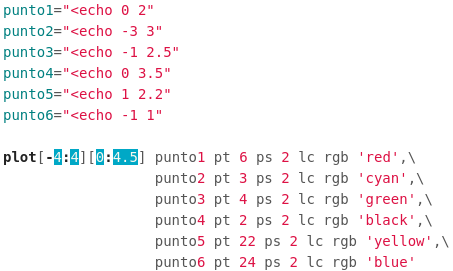
\includegraphics[scale=0.50]{screen1.png} 
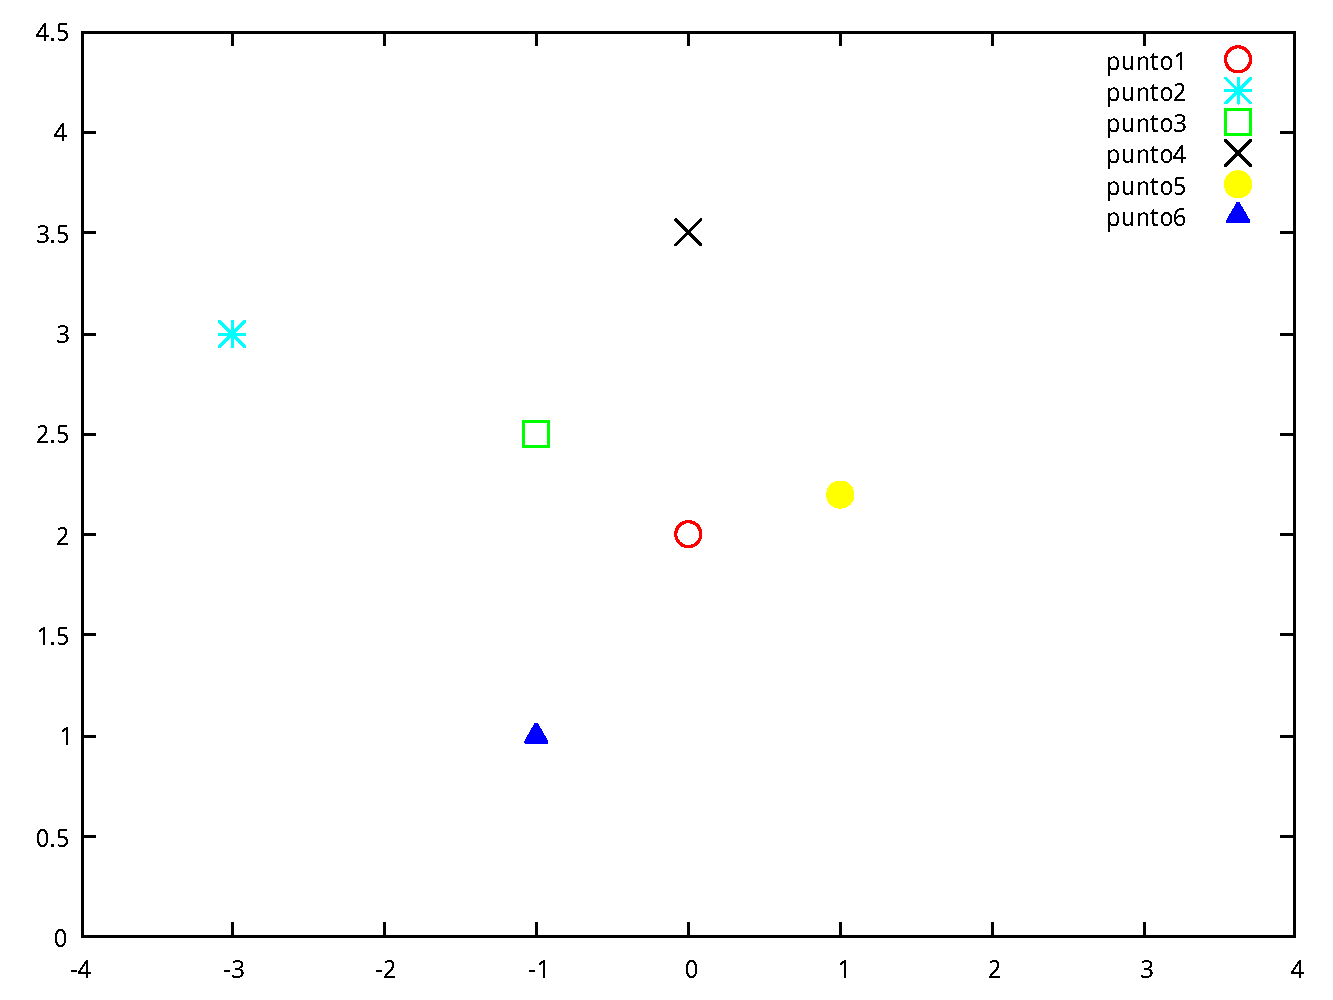
\includegraphics[scale=0.40]{ejemplo1.pdf}\\

\textbf{Ploteo de funciones}\\
 
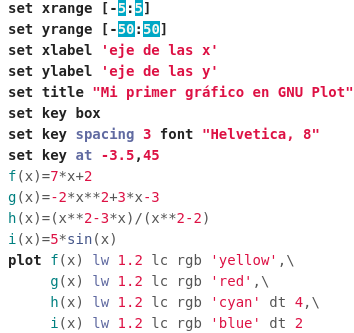
\includegraphics[scale=0.50]{screen2.png}  
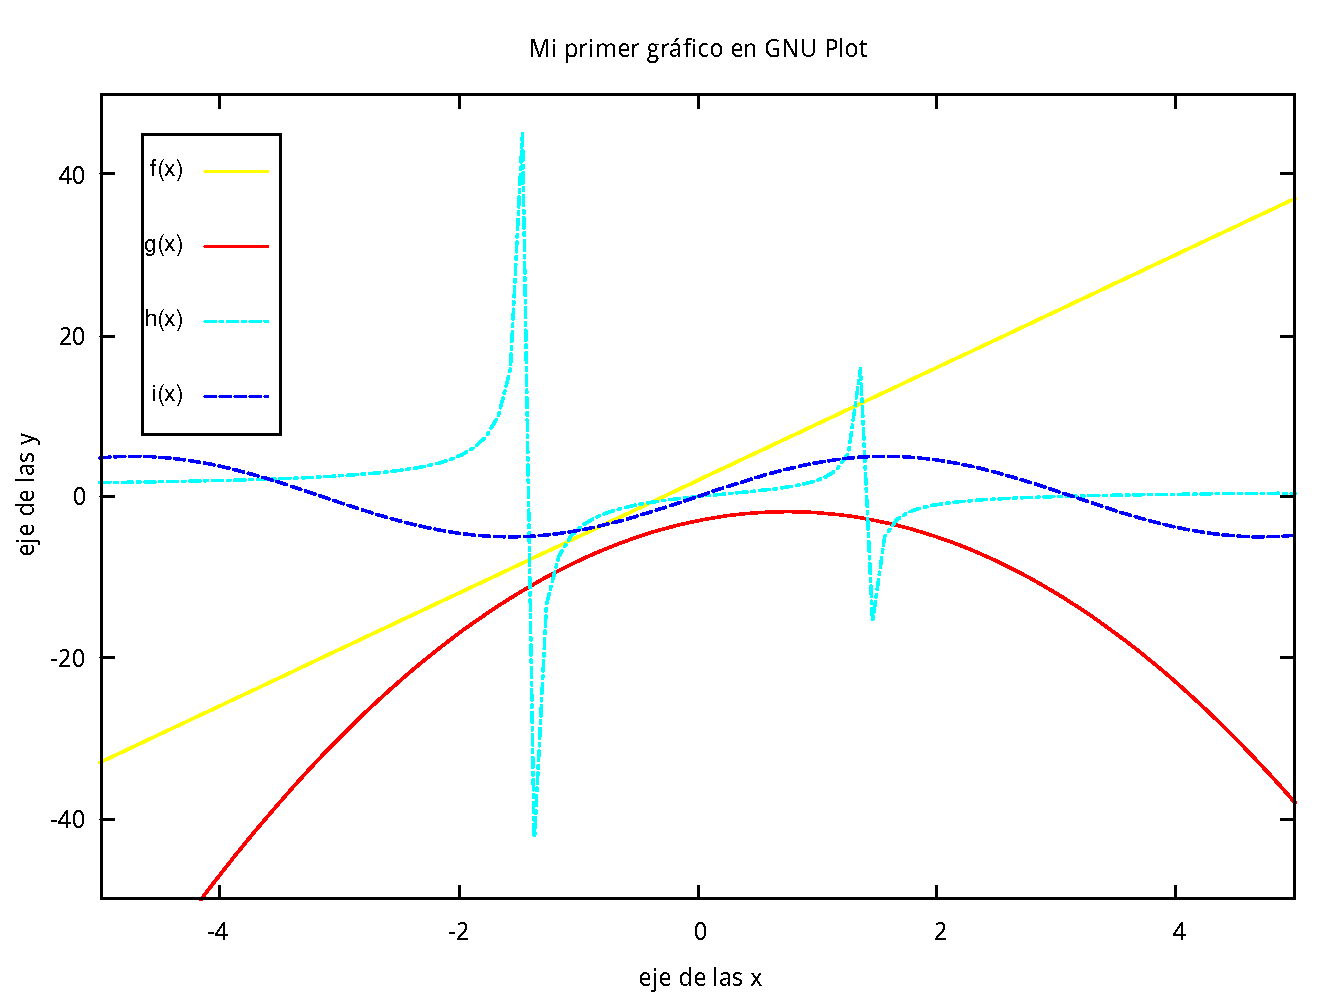
\includegraphics[scale=0.40]{ejemplo3.pdf}\\ 

\newpage
\textbf{Ejemplo práctico 1}\\

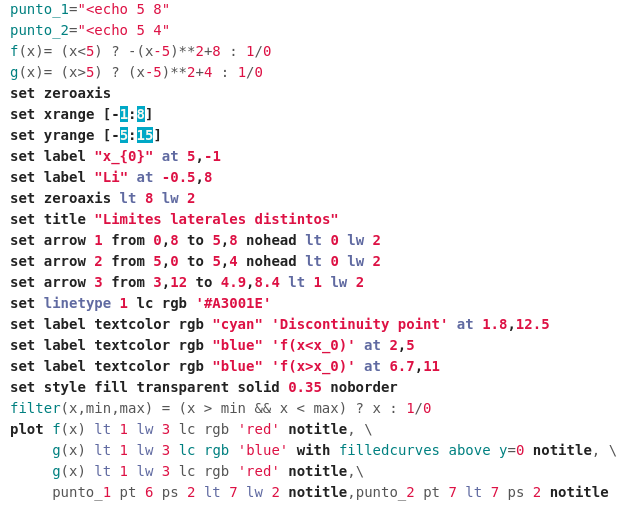
\includegraphics[scale=0.43]{screen3.png}  
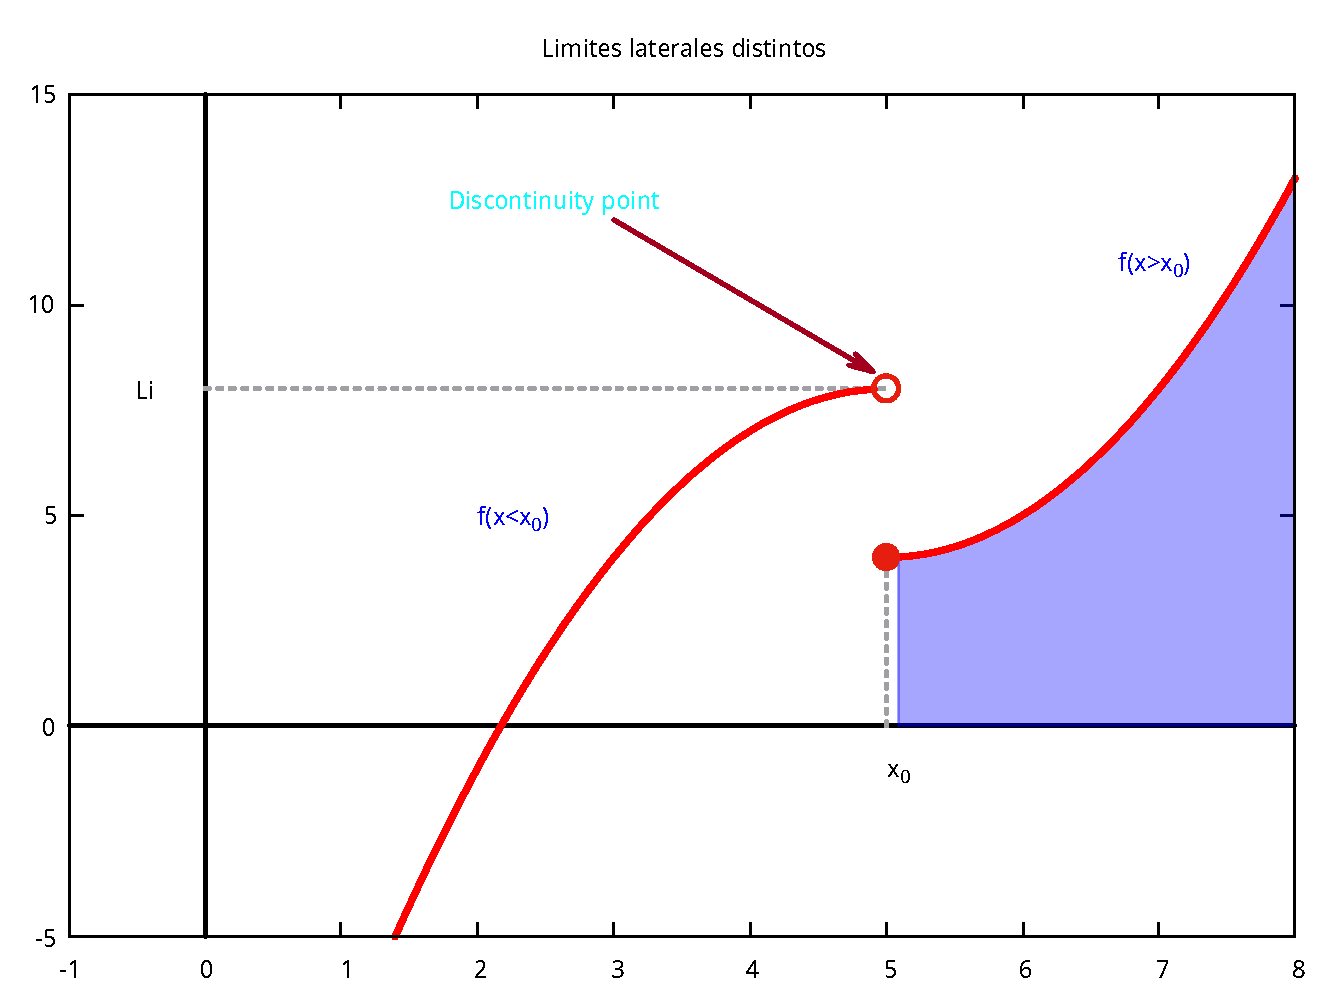
\includegraphics[scale=0.40]{ejemplo4.pdf}\\ 

\textbf{Ejemplo práctico 2}\\

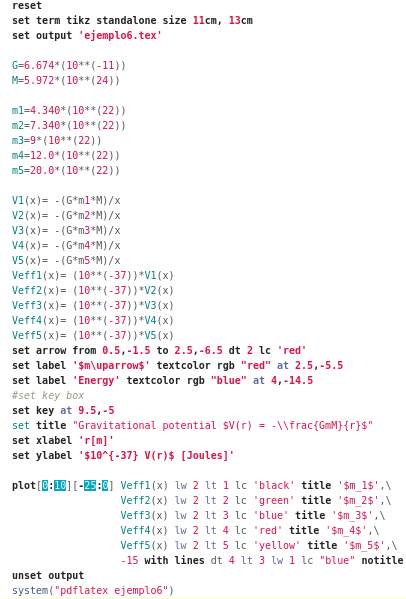
\includegraphics[scale=0.40]{screen4.png}  
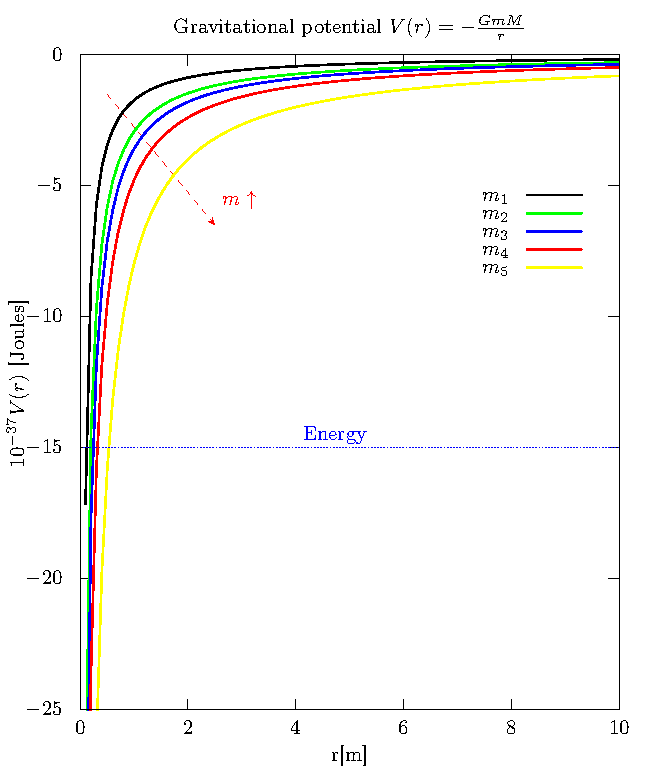
\includegraphics[scale=0.65]{ejemplo6.pdf}\\ 

\textbf{Ejemplo práctico 3}\\

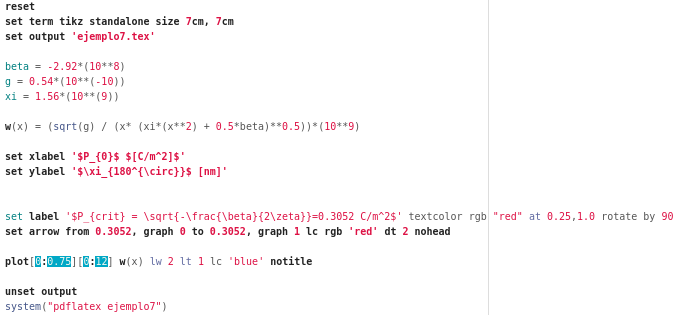
\includegraphics[scale=0.50]{screen5.png}
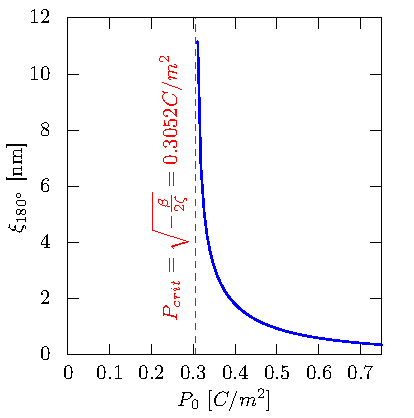
\includegraphics[scale=0.80]{ejemplo7.pdf}
\newpage
\textbf{Ejemplo práctico 4}\\


\includegraphics[scale=0.50]{screen6.png}
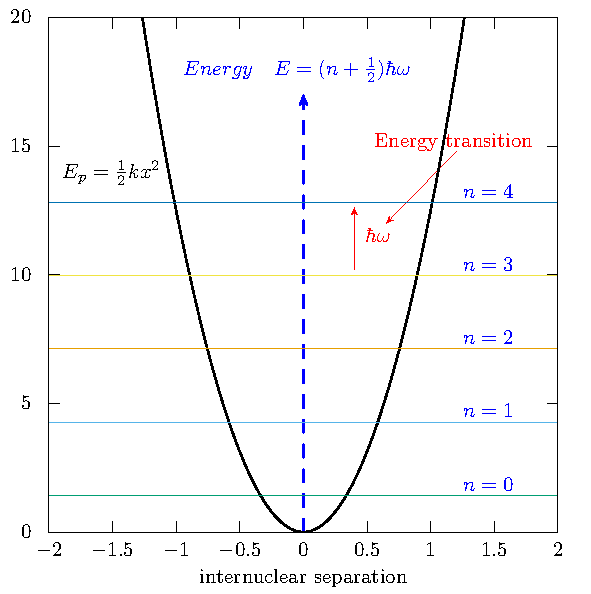
\includegraphics[scale=0.80]{ejemplo12.pdf}\\   

\textbf{Ejemplo práctico 5}\\

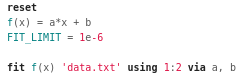
\includegraphics[scale=0.50]{screen8.png}\\
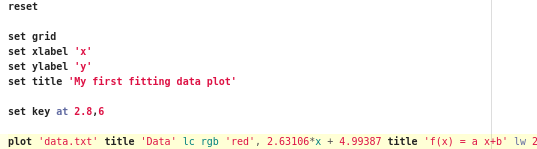
\includegraphics[scale=0.50]{screen9.png}
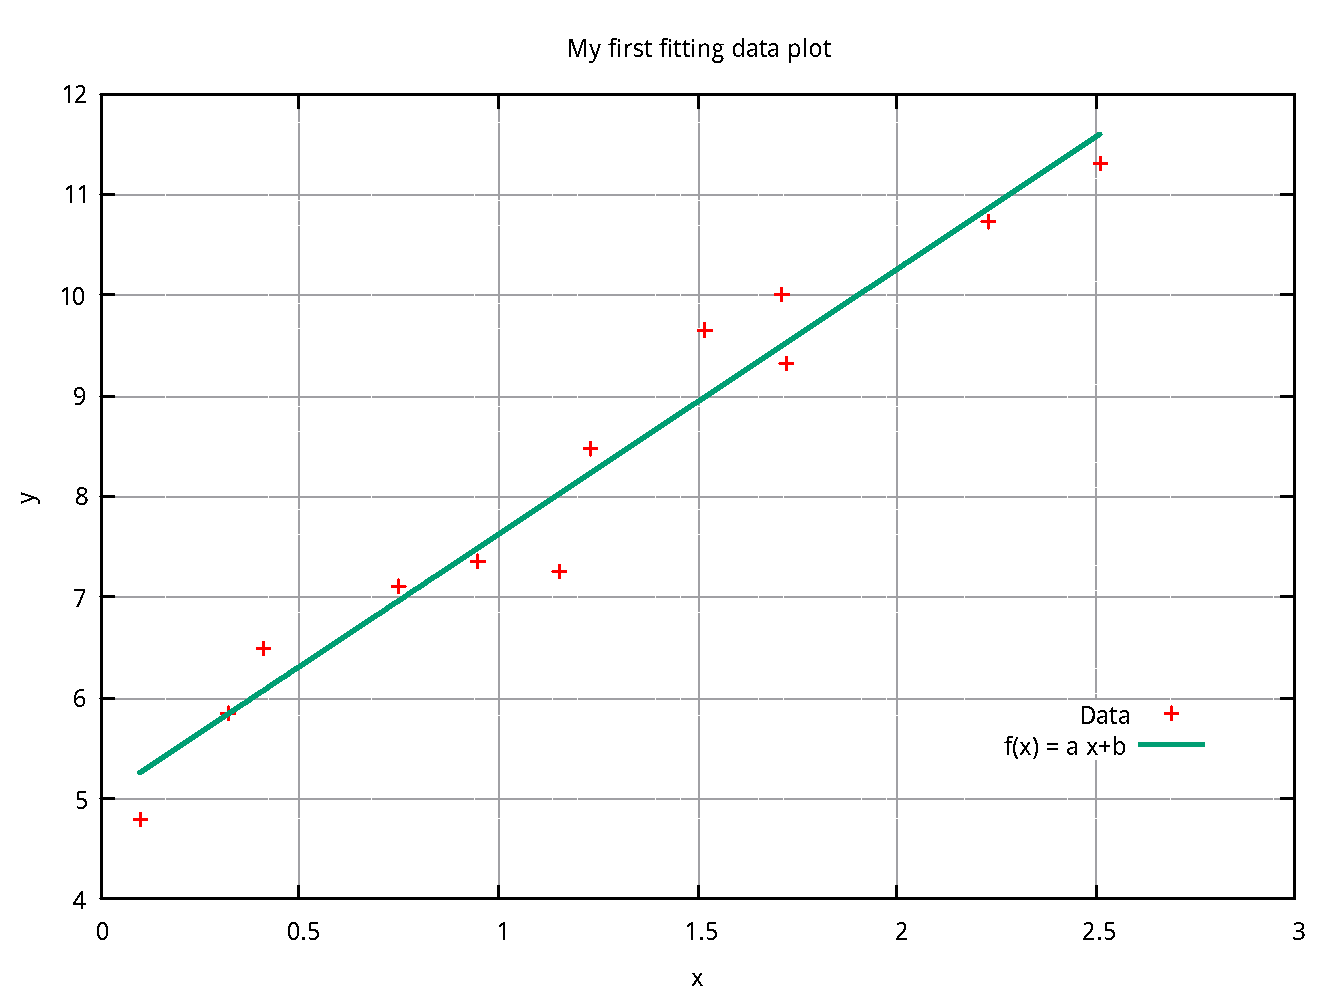
\includegraphics[scale=0.40]{ejemplo8.pdf}\\

\textbf{Ejemplo práctico 6}\\

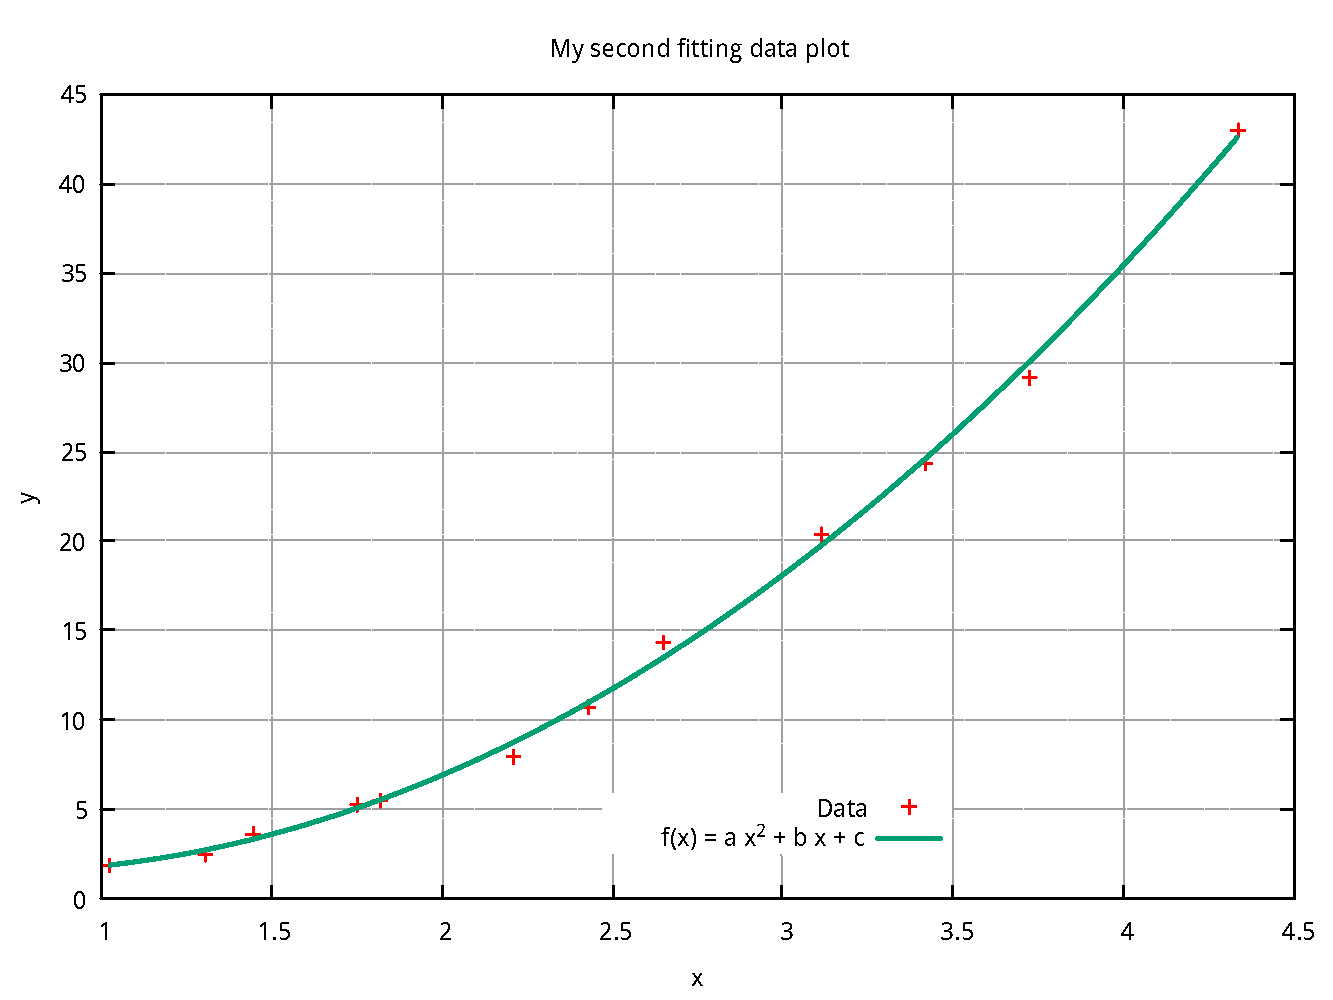
\includegraphics[scale=0.40]{ejemplo9.pdf}
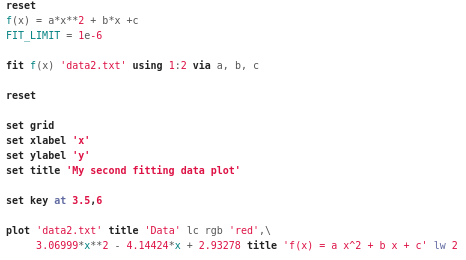
\includegraphics[scale=0.55]{screen10.png}\\

\textbf{Ejemplo práctico 7}

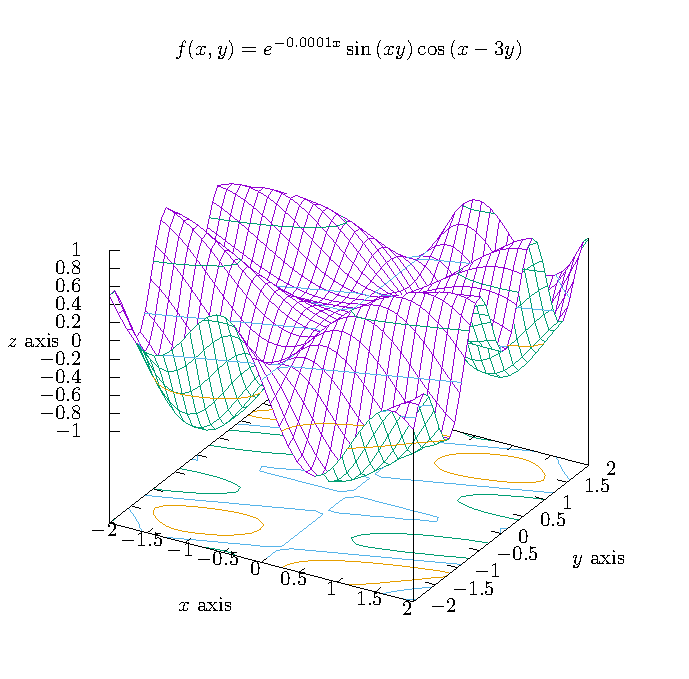
\includegraphics[scale=0.8]{ejemplo10.pdf}
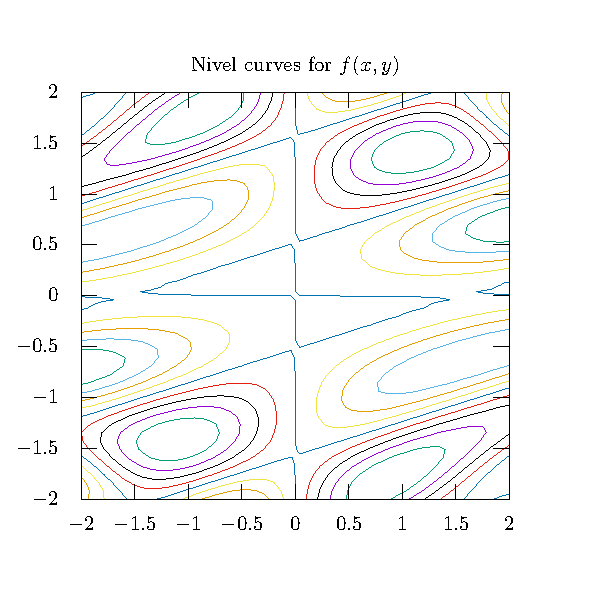
\includegraphics[scale=0.8]{ejemplo11.pdf}\\
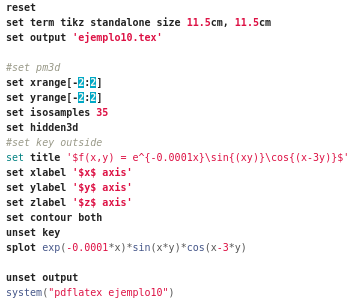
\includegraphics[scale=0.6]{screen11.png}
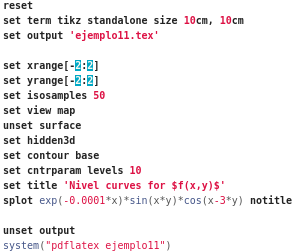
\includegraphics[scale=0.6]{screen12.png}\\*

\textbf{Ejemplo práctico 8}

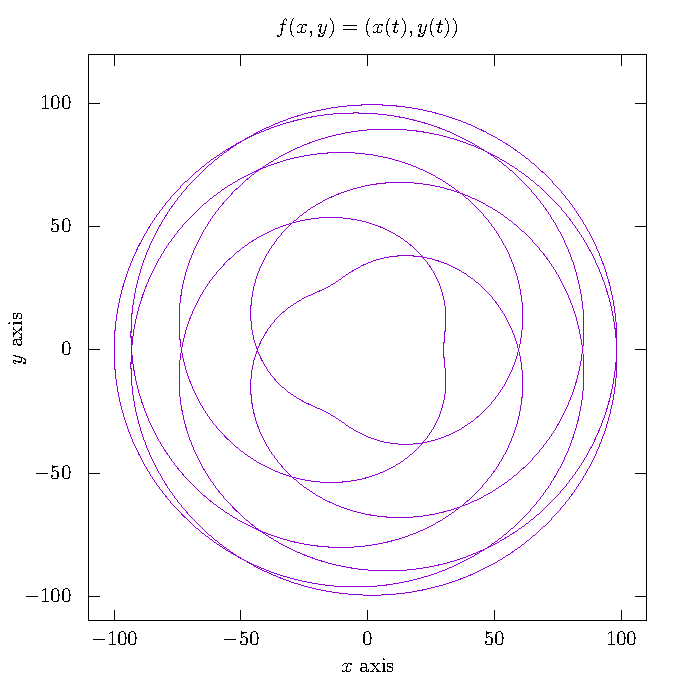
\includegraphics[scale=0.50]{ejemplo15.pdf}
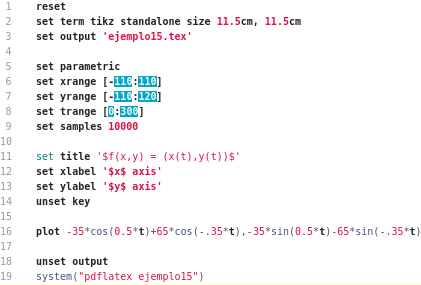
\includegraphics[scale=0.6]{screen19.png}

\newpage
\textbf{Ejemplo práctico 9}

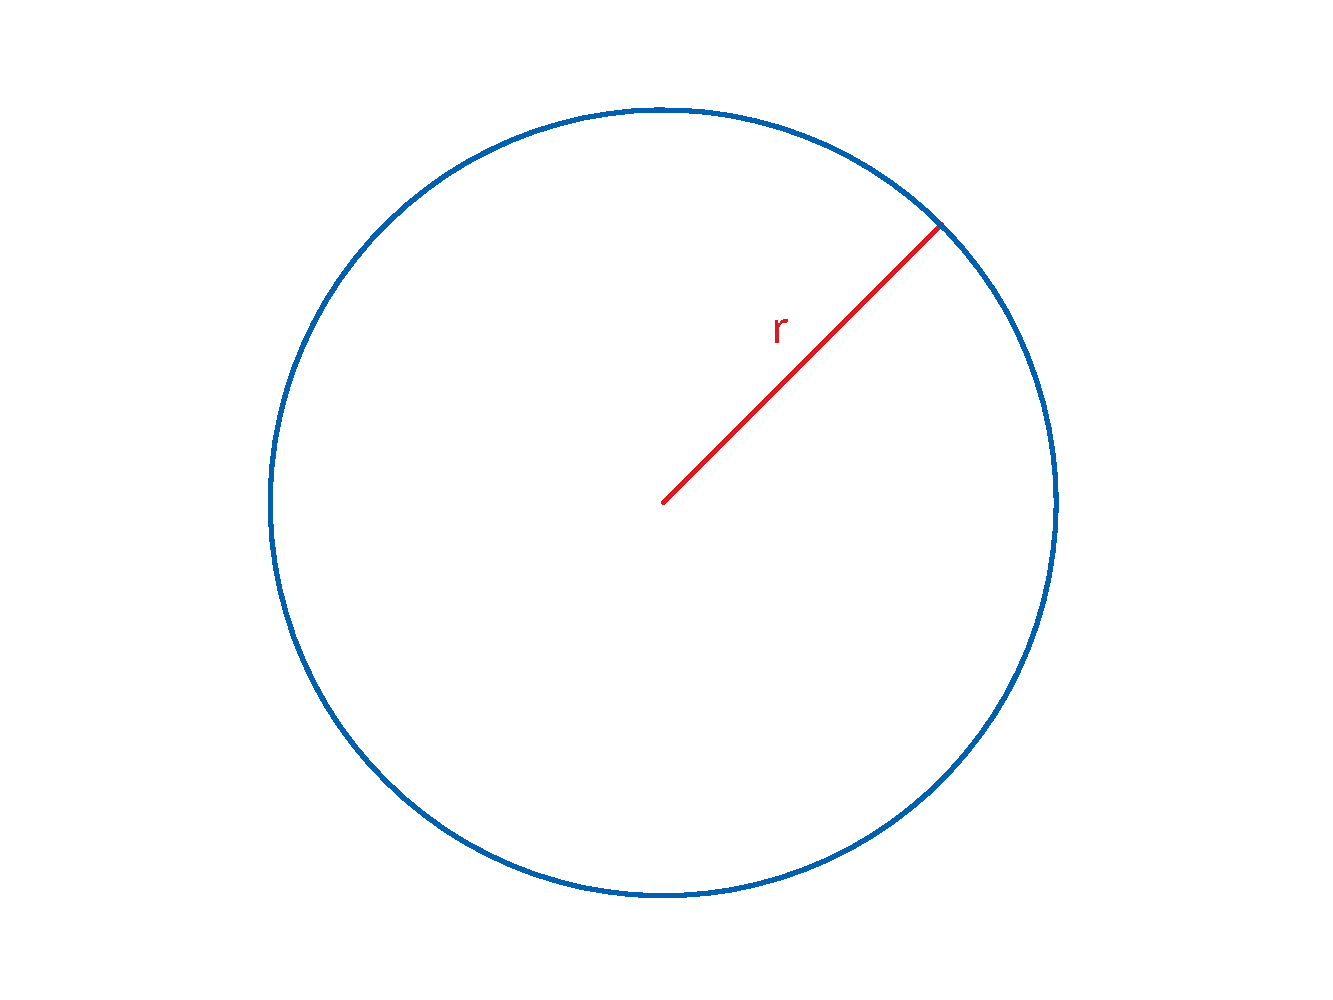
\includegraphics[scale=0.35]{ejemplo13.pdf}
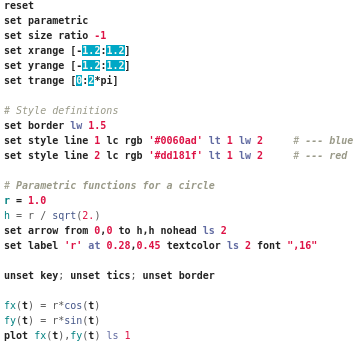
\includegraphics[scale=0.45]{screen20.png}

\textbf{Ejemplo práctico 10}

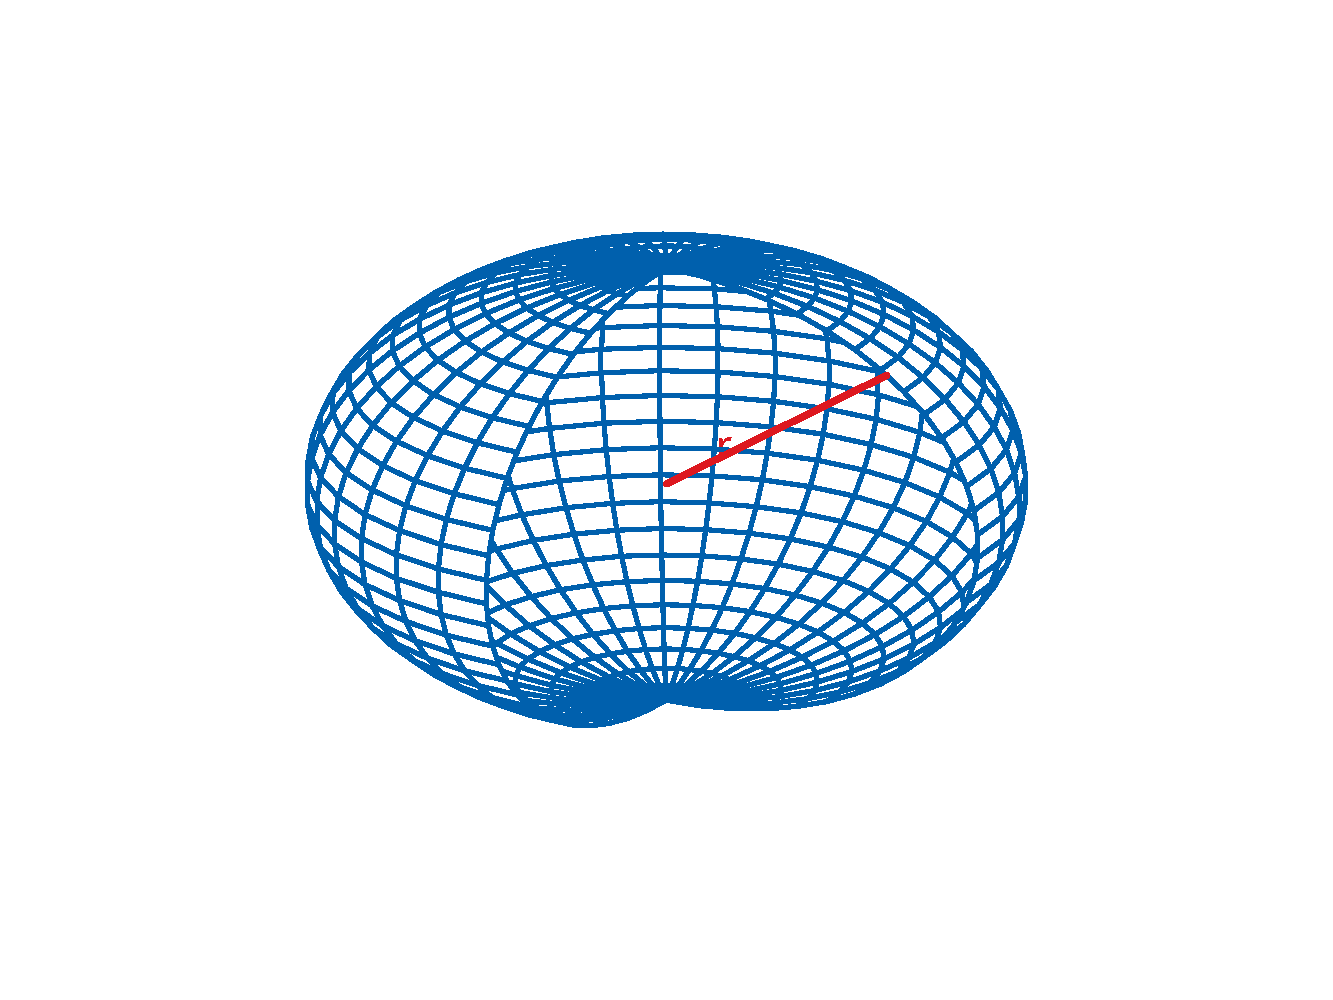
\includegraphics[scale=0.35]{ejemplo14.pdf}
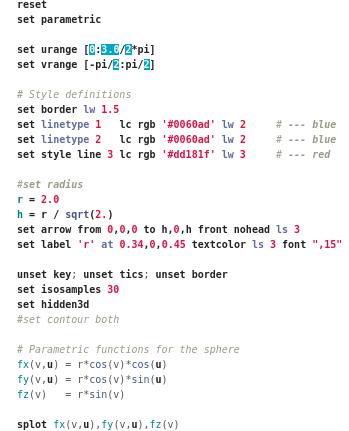
\includegraphics[scale=0.45]{screen21.png}



\newpage
\section{Ejercicios de prática}

\textbf{Ejercicio de práctica 1}\\*

La ley de Curie-Weiss describe la susceptibilidad magnética $\chi$ de un ferromagneto en la región paramagnética sobre el punto de Curie $\Theta_{C}$, o, en general, en un material casi idealmente paramagnético en el que las interacciones entre momentos magnéticos hacen que se desvíe de la ley de Curie: 

\begin{eqnarray*}
\chi(T) = \frac{C}{(T-\Theta_{C})}.
\end{eqnarray*}

Hacer un plot de la Ley de Curie para un ferromagneto que posee los siguientes valores: $C = 91.936 K$ y $\Theta_{C} = 278.5 K$.\\*

\textit{Solución}:

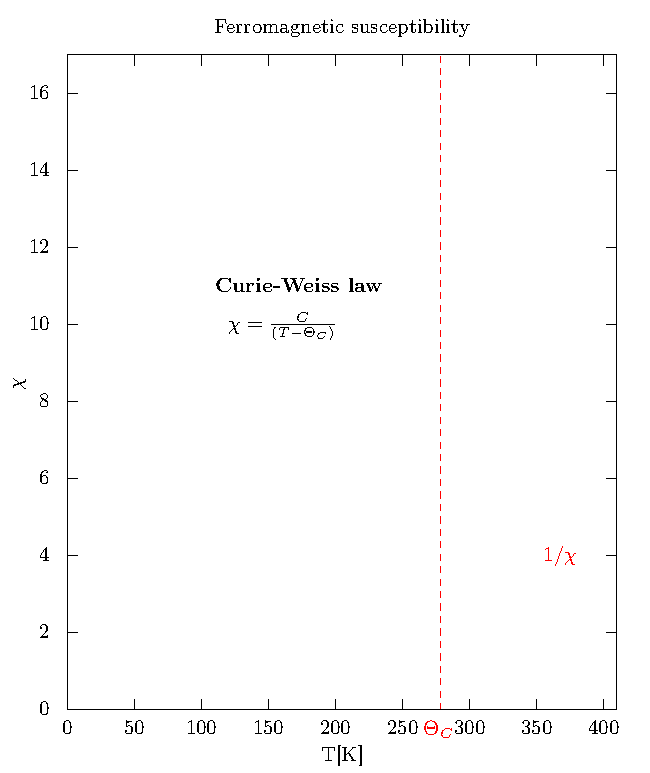
\includegraphics[scale=0.60]{ejercicio1.pdf}\\

\textbf{Potencial central}\\*

Potencial efectivo para una fuerza central similar a la gravitatoria generado por dos objetos materiales de masas $m_1$ y $m_2$ viene dado por

\begin{eqnarray*}
V_{eff} = V_{grav}(r)+V_{cf}(r)=-\frac{G m_1 m_2}{r}+\frac{L^2}{\mu r^2}
\end{eqnarray*}
donde $G$ es la constante universal de gravitación y $\mu = (m_1 m_2)/(m_1+m_2)$ la masa efectiva. Por facilidad considere $m_1=1$, $m_2=3$, $L=7$ y $G=100$ y realize un gráfico ilustrativo del potencial efectivo.\\*

\textit{Solución}:

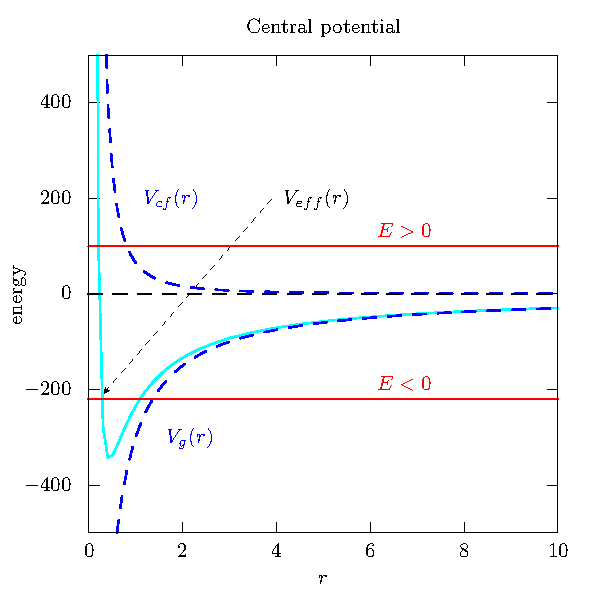
\includegraphics[scale=0.75]{ejercicio2.pdf}\\

\textbf{Fitting plot}\\*

En un experimento de cinemática se ha recolectado los siguientes datos:\\*

\begin{center}
\begin{tabular}{|c|c|}
\hline 
{\bf t[seg]} & {\bf x[m]} \\ 
\hline
0.001 & 1.842 \\ 
\hline 
0.513 & 1.765 \\ 
\hline 
1.234 & 5.785 \\ 
\hline 
2.341 & 19.672 \\ 
\hline 
2.451 & 26.412 \\ 
\hline 
3.312 & 43.987\\
\hline
3.555 & 54.671\\
\hline
4.101 & 70.011\\
\hline
4.212 & 77.621\\
\hline
5.511 & 123.345\\
\hline
\end{tabular} 
\end{center}

Encuentre las funciones $f(x)=ax^2+bx+c$ y $g(x)=\sqrt{ax^2+bx+c}$ que se ajustan a estos datos mediante gnuplot y graficarlas.\\*

\textit{Solución}:

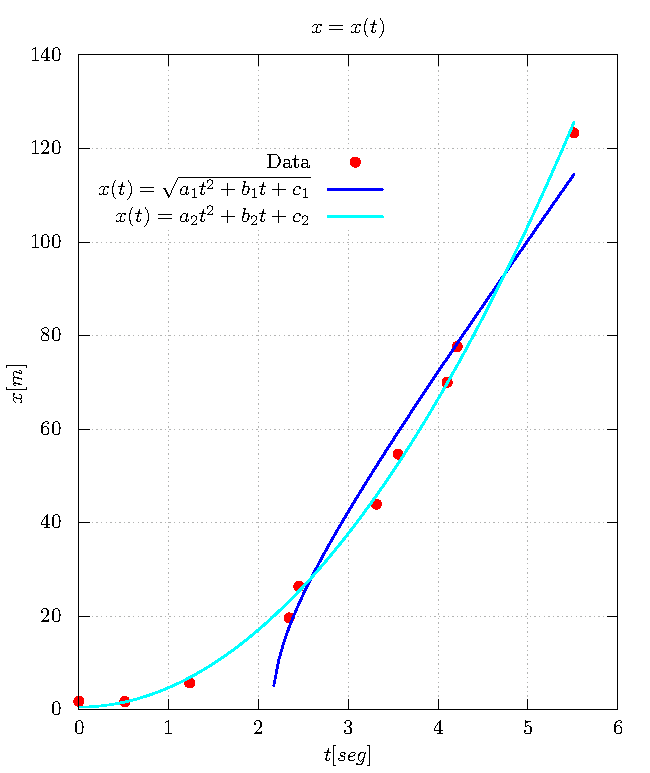
\includegraphics[scale=0.60]{ejercicio3.pdf}\\

\textbf{3D plots}\\*

Realize la gráfica de las funciones $f(x,y)=\sqrt{100-x^2-y^2}$ y $g(x,y)= x-y$ y una gráfica de sus contornos.\\*

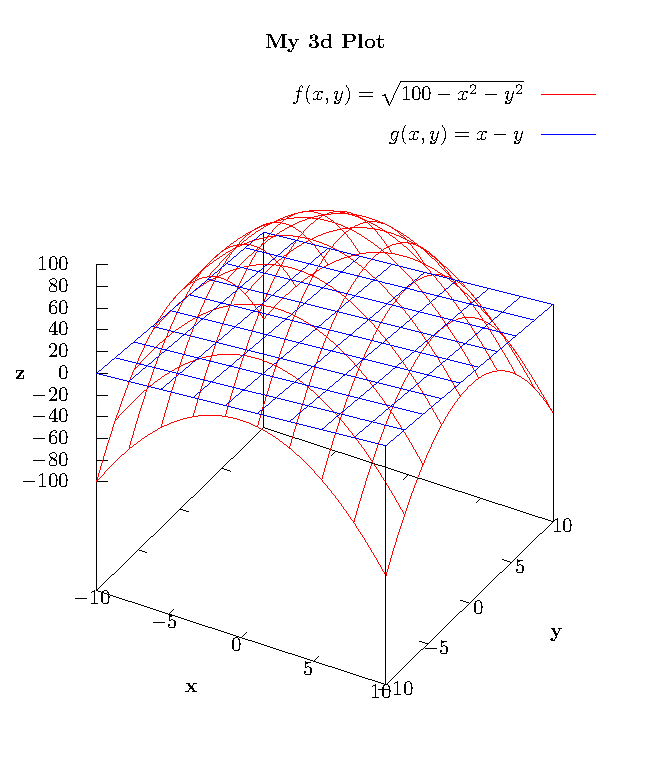
\includegraphics[scale=0.70]{ejercicio4.pdf}
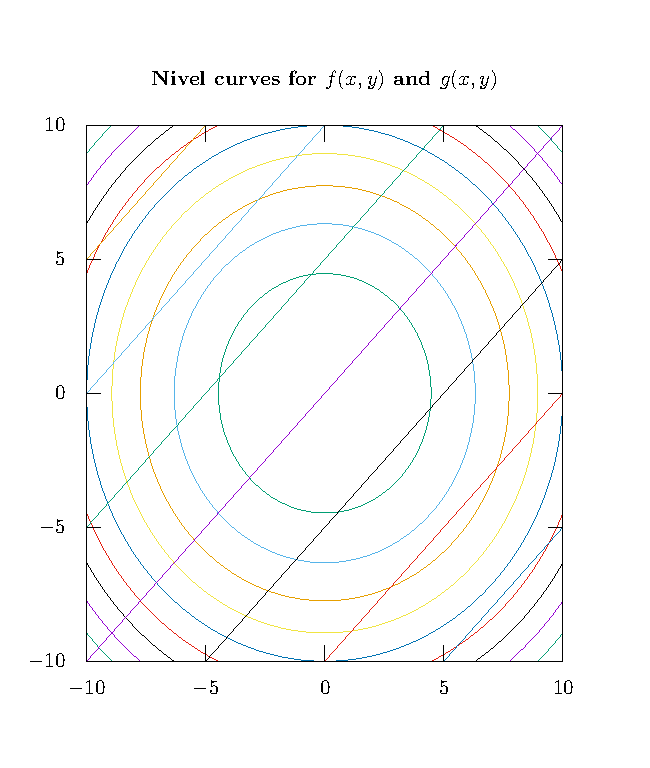
\includegraphics[scale=0.70]{ejercicio4a.pdf}

\newpage

\section{Soluciones de los ejercicios}

\textbf{Ejercicio 1}\\

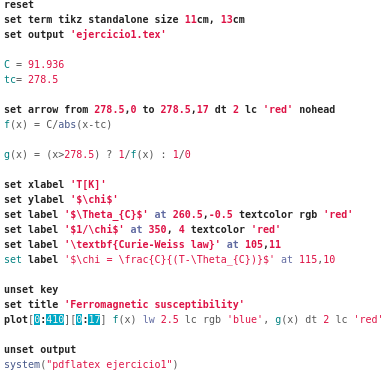
\includegraphics[scale=0.75]{screen13.png}\\

\textbf{Ejercicio 2}\\

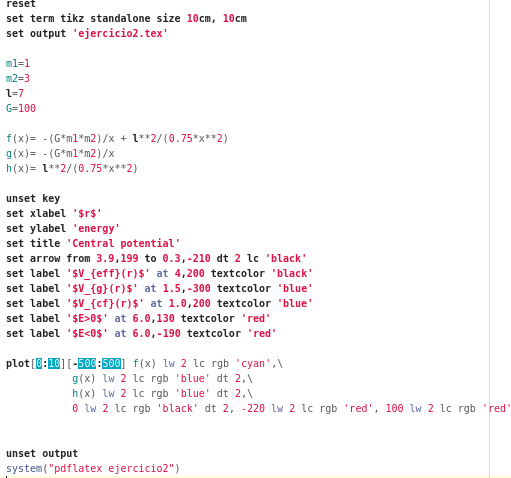
\includegraphics[scale=0.75]{screen14.png}\\
\newpage
\textbf{Ejercicio 3}\\

Primero creo un archivo de texto con los datos. Luego ejecuto el siguiente script para obtener las funciones de interpolación.\\*

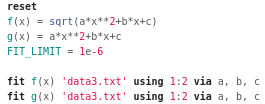
\includegraphics[scale=0.75]{screen15.png}\\

Y luego ejecuto el siguiente script.\\*

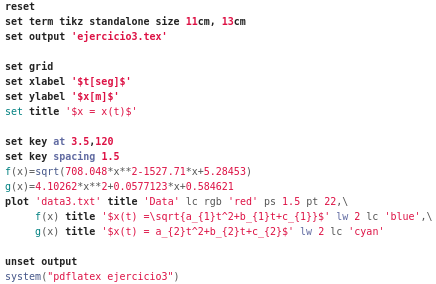
\includegraphics[scale=0.75]{screen16.png}\\

\textbf{Ejercicio 4}\\

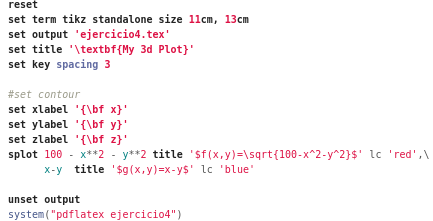
\includegraphics[scale=0.65]{screen17.png}
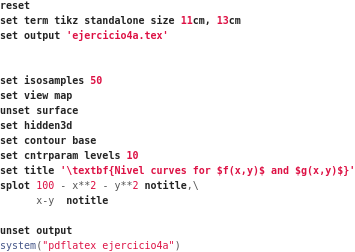
\includegraphics[scale=0.65]{screen18.png}

\end{document}
